% Created by tikzDevice version 0.6.2 on 2012-04-22 09:19:34
% !TEX encoding = UTF-8 Unicode
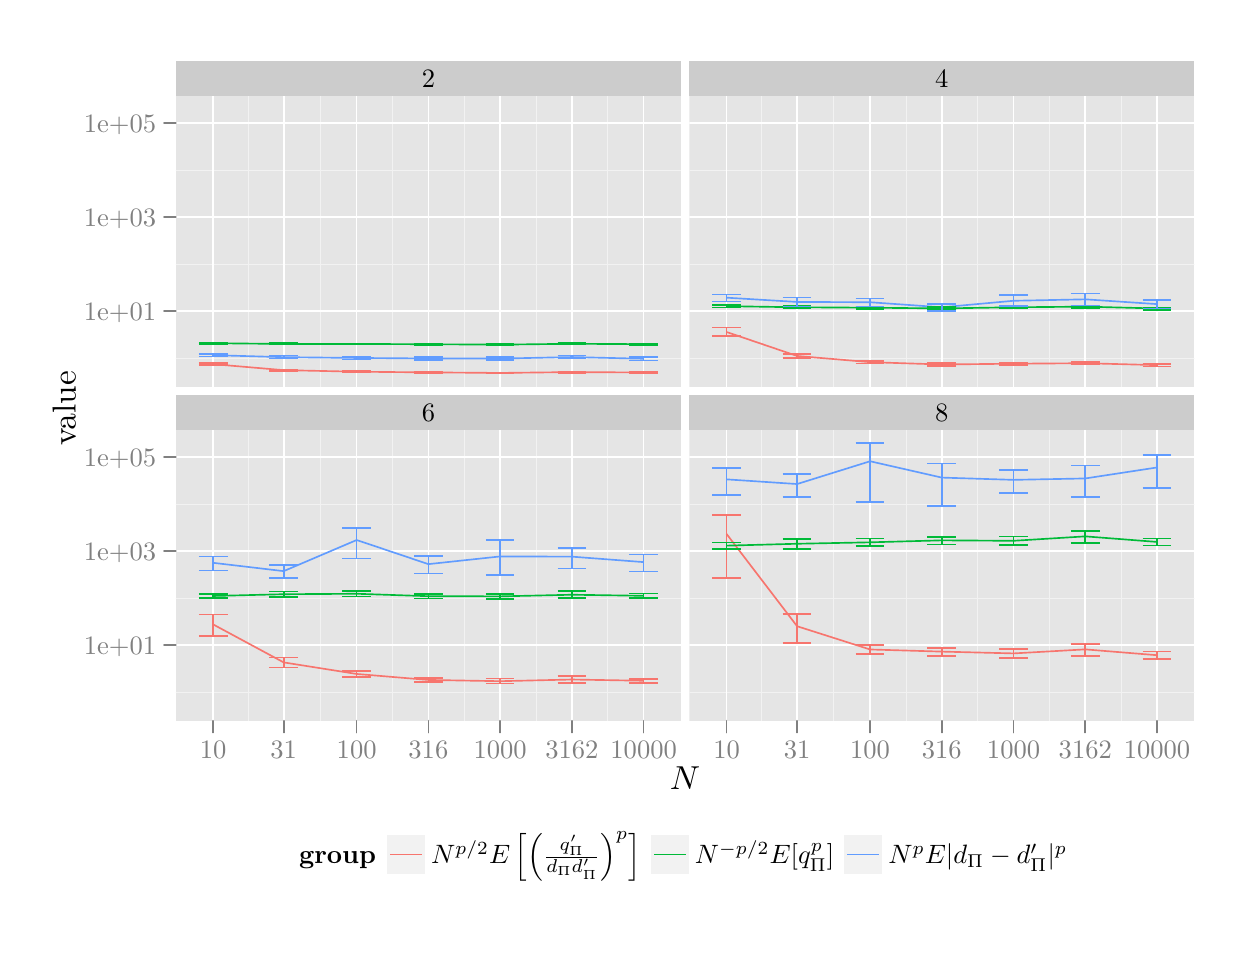
\begin{tikzpicture}[x=1pt,y=1pt]
\definecolor[named]{drawColor}{rgb}{0.00,0.00,0.00}
\definecolor[named]{fillColor}{rgb}{1.00,1.00,1.00}
\fill[color=fillColor,fill opacity=0.00,] (0,0) rectangle (433.62,325.21);
\begin{scope}
\path[clip] (  0.00,  0.00) rectangle (433.62,325.21);
\definecolor[named]{drawColor}{rgb}{0.41,0.16,0.58}
\end{scope}
\begin{scope}
\path[clip] (  0.00,  0.00) rectangle (433.62,325.21);
\definecolor[named]{drawColor}{rgb}{0.41,0.16,0.58}
\end{scope}
\begin{scope}
\path[clip] (  0.00,  0.00) rectangle (433.62,325.21);
\definecolor[named]{drawColor}{rgb}{0.41,0.16,0.58}
\end{scope}
\begin{scope}
\path[clip] (  0.00,  0.00) rectangle (433.62,325.21);
\definecolor[named]{drawColor}{rgb}{0.41,0.16,0.58}
\end{scope}
\begin{scope}
\path[clip] (  0.00,  0.00) rectangle (433.62,325.21);
\definecolor[named]{drawColor}{rgb}{0.41,0.16,0.58}
\end{scope}
\begin{scope}
\path[clip] (  0.00,  0.00) rectangle (433.62,325.21);
\definecolor[named]{drawColor}{rgb}{0.41,0.16,0.58}
\end{scope}
\begin{scope}
\path[clip] (  0.00,  0.00) rectangle (433.62,325.21);
\definecolor[named]{drawColor}{rgb}{0.41,0.16,0.58}
\end{scope}
\begin{scope}
\path[clip] (  0.00,  0.00) rectangle (433.62,325.21);
\definecolor[named]{drawColor}{rgb}{0.41,0.16,0.58}
\end{scope}
\begin{scope}
\path[clip] ( 53.55,195.47) rectangle (236.06,300.54);
\definecolor[named]{drawColor}{rgb}{0.41,0.16,0.58}
\end{scope}
\begin{scope}
\path[clip] (  0.00,  0.00) rectangle (433.62,325.21);
\definecolor[named]{drawColor}{rgb}{0.41,0.16,0.58}
\end{scope}
\begin{scope}
\path[clip] (239.07,195.47) rectangle (421.58,300.54);
\definecolor[named]{drawColor}{rgb}{0.41,0.16,0.58}
\end{scope}
\begin{scope}
\path[clip] (  0.00,  0.00) rectangle (433.62,325.21);
\definecolor[named]{drawColor}{rgb}{0.41,0.16,0.58}
\end{scope}
\begin{scope}
\path[clip] ( 53.55, 74.76) rectangle (236.06,179.83);
\definecolor[named]{drawColor}{rgb}{0.41,0.16,0.58}
\end{scope}
\begin{scope}
\path[clip] (  0.00,  0.00) rectangle (433.62,325.21);
\definecolor[named]{drawColor}{rgb}{0.41,0.16,0.58}
\end{scope}
\begin{scope}
\path[clip] (239.07, 74.76) rectangle (421.58,179.83);
\definecolor[named]{drawColor}{rgb}{0.41,0.16,0.58}
\end{scope}
\begin{scope}
\path[clip] (  0.00,  0.00) rectangle (433.62,325.21);
\definecolor[named]{drawColor}{rgb}{0.41,0.16,0.58}
\end{scope}
\begin{scope}
\path[clip] (  0.00,  0.00) rectangle (433.62,325.21);
\definecolor[named]{drawColor}{rgb}{0.41,0.16,0.58}
\end{scope}
\begin{scope}
\path[clip] (  0.00,  0.00) rectangle (433.62,325.21);
\definecolor[named]{drawColor}{rgb}{0.41,0.16,0.58}
\end{scope}
\begin{scope}
\path[clip] (  0.00,  0.00) rectangle (433.62,325.21);
\definecolor[named]{drawColor}{rgb}{0.41,0.16,0.58}
\end{scope}
\begin{scope}
\path[clip] (  0.00,  0.00) rectangle (433.62,325.21);
\definecolor[named]{drawColor}{rgb}{0.41,0.16,0.58}
\end{scope}
\begin{scope}
\path[clip] (  0.00,  0.00) rectangle (433.62,325.21);
\definecolor[named]{drawColor}{rgb}{0.41,0.16,0.58}
\end{scope}
\begin{scope}
\path[clip] (  0.00,  0.00) rectangle (433.62,325.21);
\definecolor[named]{drawColor}{rgb}{0.41,0.16,0.58}
\end{scope}
\begin{scope}
\path[clip] (  0.00,  0.00) rectangle (433.62,325.21);
\definecolor[named]{drawColor}{rgb}{0.41,0.16,0.58}
\end{scope}
\begin{scope}
\path[clip] (  0.00,  0.00) rectangle (433.62,325.21);
\definecolor[named]{drawColor}{rgb}{0.41,0.16,0.58}
\end{scope}
\begin{scope}
\path[clip] (  0.00,  0.00) rectangle (433.62,325.21);
\definecolor[named]{drawColor}{rgb}{0.41,0.16,0.58}
\end{scope}
\begin{scope}
\path[clip] (  0.00,  0.00) rectangle (433.62,325.21);
\definecolor[named]{drawColor}{rgb}{0.41,0.16,0.58}
\end{scope}
\begin{scope}
\path[clip] (  0.00,  0.00) rectangle (433.62,325.21);
\definecolor[named]{drawColor}{rgb}{0.41,0.16,0.58}
\end{scope}
\begin{scope}
\path[clip] (  0.00,  0.00) rectangle (433.62,325.21);
\definecolor[named]{drawColor}{rgb}{0.41,0.16,0.58}
\end{scope}
\begin{scope}
\path[clip] (  0.00,  0.00) rectangle (433.62,325.21);
\definecolor[named]{drawColor}{rgb}{0.41,0.16,0.58}
\end{scope}
\begin{scope}
\path[clip] (  0.00,  0.00) rectangle (433.62,325.21);
\definecolor[named]{drawColor}{rgb}{0.41,0.16,0.58}
\end{scope}
\begin{scope}
\path[clip] (  0.00,  0.00) rectangle (433.62,325.21);
\definecolor[named]{drawColor}{rgb}{0.41,0.16,0.58}
\end{scope}
\begin{scope}
\path[clip] (  0.00,  0.00) rectangle (433.62,325.21);
\definecolor[named]{drawColor}{rgb}{0.41,0.16,0.58}
\end{scope}
\begin{scope}
\path[clip] (  0.00,  0.00) rectangle (433.62,325.21);
\definecolor[named]{drawColor}{rgb}{0.41,0.16,0.58}
\end{scope}
\begin{scope}
\path[clip] (  0.00,  0.00) rectangle (433.62,325.21);
\definecolor[named]{drawColor}{rgb}{0.41,0.16,0.58}
\end{scope}
\begin{scope}
\path[clip] (  0.00,  0.00) rectangle (433.62,325.21);
\definecolor[named]{drawColor}{rgb}{0.41,0.16,0.58}
\end{scope}
\begin{scope}
\path[clip] (  0.00,  0.00) rectangle (433.62,325.21);
\definecolor[named]{drawColor}{rgb}{0.41,0.16,0.58}
\end{scope}
\begin{scope}
\path[clip] (  0.00,  0.00) rectangle (433.62,325.21);
\definecolor[named]{drawColor}{rgb}{0.41,0.16,0.58}
\end{scope}
\begin{scope}
\path[clip] (  0.00,  0.00) rectangle (433.62,325.21);
\definecolor[named]{drawColor}{rgb}{0.41,0.16,0.58}
\end{scope}
\begin{scope}
\path[clip] (  0.00,  0.00) rectangle (433.62,325.21);
\definecolor[named]{drawColor}{rgb}{0.41,0.16,0.58}
\end{scope}
\begin{scope}
\path[clip] (  0.00,  0.00) rectangle (433.62,325.21);
\definecolor[named]{drawColor}{rgb}{0.41,0.16,0.58}
\end{scope}
\begin{scope}
\path[clip] (  0.00,  0.00) rectangle (433.62,325.21);
\definecolor[named]{drawColor}{rgb}{0.41,0.16,0.58}
\end{scope}
\begin{scope}
\path[clip] (  0.00,  0.00) rectangle (433.62,325.21);
\definecolor[named]{drawColor}{rgb}{0.41,0.16,0.58}
\end{scope}
\begin{scope}
\path[clip] (  0.00,  0.00) rectangle (433.62,325.21);
\definecolor[named]{drawColor}{rgb}{0.41,0.16,0.58}
\end{scope}
\begin{scope}
\path[clip] (  0.00,  0.00) rectangle (433.62,325.21);
\definecolor[named]{drawColor}{rgb}{0.41,0.16,0.58}
\end{scope}
\begin{scope}
\path[clip] (  0.00,  0.00) rectangle (433.62,325.21);
\definecolor[named]{drawColor}{rgb}{0.41,0.16,0.58}
\end{scope}
\begin{scope}
\path[clip] (  0.00,  0.00) rectangle (433.62,325.21);
\definecolor[named]{drawColor}{rgb}{0.41,0.16,0.58}
\end{scope}
\begin{scope}
\path[clip] (  0.00,  0.00) rectangle (433.62,325.21);
\definecolor[named]{drawColor}{rgb}{0.41,0.16,0.58}
\end{scope}
\begin{scope}
\path[clip] (  0.00,  0.00) rectangle (433.62,325.21);
\definecolor[named]{drawColor}{rgb}{0.41,0.16,0.58}
\end{scope}
\begin{scope}
\path[clip] (  0.00,  0.00) rectangle (433.62,325.21);
\definecolor[named]{drawColor}{rgb}{0.41,0.16,0.58}
\definecolor[named]{fillColor}{rgb}{1.00,1.00,1.00}

\draw[fill=fillColor,draw opacity=0.00,] (  0.00,  0.00) rectangle (433.62,325.21);
\end{scope}
\begin{scope}
\path[clip] (  0.00,  0.00) rectangle (433.62,325.21);
\definecolor[named]{drawColor}{rgb}{0.41,0.16,0.58}
\end{scope}
\begin{scope}
\path[clip] ( 53.55,195.47) rectangle (236.06,300.54);
\definecolor[named]{drawColor}{rgb}{0.41,0.16,0.58}
\definecolor[named]{fillColor}{rgb}{0.90,0.90,0.90}

\draw[fill=fillColor,draw opacity=0.00,] ( 53.55,195.47) rectangle (236.06,300.54);
\definecolor[named]{drawColor}{rgb}{0.95,0.95,0.95}

\draw[color=drawColor,line width= 0.3pt,line cap=round,line join=round,fill opacity=0.00,] ( 53.55,205.77) --
	(236.06,205.77);

\draw[color=drawColor,line width= 0.3pt,line cap=round,line join=round,fill opacity=0.00,] ( 53.55,239.78) --
	(236.06,239.78);

\draw[color=drawColor,line width= 0.3pt,line cap=round,line join=round,fill opacity=0.00,] ( 53.55,273.79) --
	(236.06,273.79);

\draw[color=drawColor,line width= 0.3pt,line cap=round,line join=round,fill opacity=0.00,] ( 79.77,195.47) --
	( 79.77,300.54);

\draw[color=drawColor,line width= 0.3pt,line cap=round,line join=round,fill opacity=0.00,] (105.69,195.47) --
	(105.69,300.54);

\draw[color=drawColor,line width= 0.3pt,line cap=round,line join=round,fill opacity=0.00,] (131.83,195.47) --
	(131.83,300.54);

\draw[color=drawColor,line width= 0.3pt,line cap=round,line join=round,fill opacity=0.00,] (157.76,195.47) --
	(157.76,300.54);

\draw[color=drawColor,line width= 0.3pt,line cap=round,line join=round,fill opacity=0.00,] (183.69,195.47) --
	(183.69,300.54);

\draw[color=drawColor,line width= 0.3pt,line cap=round,line join=round,fill opacity=0.00,] (209.61,195.47) --
	(209.61,300.54);
\definecolor[named]{drawColor}{rgb}{1.00,1.00,1.00}

\draw[color=drawColor,line width= 0.6pt,line cap=round,line join=round,fill opacity=0.00,] ( 53.55,222.77) --
	(236.06,222.77);

\draw[color=drawColor,line width= 0.6pt,line cap=round,line join=round,fill opacity=0.00,] ( 53.55,256.78) --
	(236.06,256.78);

\draw[color=drawColor,line width= 0.6pt,line cap=round,line join=round,fill opacity=0.00,] ( 53.55,290.80) --
	(236.06,290.80);

\draw[color=drawColor,line width= 0.6pt,line cap=round,line join=round,fill opacity=0.00,] ( 67.03,195.47) --
	( 67.03,300.54);

\draw[color=drawColor,line width= 0.6pt,line cap=round,line join=round,fill opacity=0.00,] ( 92.51,195.47) --
	( 92.51,300.54);

\draw[color=drawColor,line width= 0.6pt,line cap=round,line join=round,fill opacity=0.00,] (118.88,195.47) --
	(118.88,300.54);

\draw[color=drawColor,line width= 0.6pt,line cap=round,line join=round,fill opacity=0.00,] (144.79,195.47) --
	(144.79,300.54);

\draw[color=drawColor,line width= 0.6pt,line cap=round,line join=round,fill opacity=0.00,] (170.73,195.47) --
	(170.73,300.54);

\draw[color=drawColor,line width= 0.6pt,line cap=round,line join=round,fill opacity=0.00,] (196.65,195.47) --
	(196.65,300.54);

\draw[color=drawColor,line width= 0.6pt,line cap=round,line join=round,fill opacity=0.00,] (222.58,195.47) --
	(222.58,300.54);
\definecolor[named]{drawColor}{rgb}{0.97,0.46,0.43}

\draw[color=drawColor,line width= 0.6pt,line join=round,fill opacity=0.00,] ( 67.03,203.62) --
	( 92.51,201.45) --
	(118.88,200.89) --
	(144.79,200.64) --
	(170.73,200.45) --
	(196.65,200.75) --
	(222.58,200.61);
\definecolor[named]{drawColor}{rgb}{0.00,0.73,0.22}

\draw[color=drawColor,line width= 0.6pt,line join=round,fill opacity=0.00,] ( 67.03,211.18) --
	( 92.51,210.93) --
	(118.88,210.93) --
	(144.79,210.81) --
	(170.73,210.67) --
	(196.65,210.98) --
	(222.58,210.84);
\definecolor[named]{drawColor}{rgb}{0.38,0.61,1.00}

\draw[color=drawColor,line width= 0.6pt,line join=round,fill opacity=0.00,] ( 67.03,206.87) --
	( 92.51,206.15) --
	(118.88,205.86) --
	(144.79,205.67) --
	(170.73,205.63) --
	(196.65,206.19) --
	(222.58,205.57);
\definecolor[named]{drawColor}{rgb}{0.97,0.46,0.43}

\draw[color=drawColor,line width= 0.6pt,line join=round,fill opacity=0.00,] ( 61.85,203.97) --
	( 72.22,203.97);

\draw[color=drawColor,line width= 0.6pt,line join=round,fill opacity=0.00,] ( 67.03,203.97) --
	( 67.03,203.29);

\draw[color=drawColor,line width= 0.6pt,line join=round,fill opacity=0.00,] ( 61.85,203.29) --
	( 72.22,203.29);

\draw[color=drawColor,line width= 0.6pt,line join=round,fill opacity=0.00,] ( 87.32,201.67) --
	( 97.69,201.67);

\draw[color=drawColor,line width= 0.6pt,line join=round,fill opacity=0.00,] ( 92.51,201.67) --
	( 92.51,201.22);

\draw[color=drawColor,line width= 0.6pt,line join=round,fill opacity=0.00,] ( 87.32,201.22) --
	( 97.69,201.22);

\draw[color=drawColor,line width= 0.6pt,line join=round,fill opacity=0.00,] (113.69,201.09) --
	(124.06,201.09);

\draw[color=drawColor,line width= 0.6pt,line join=round,fill opacity=0.00,] (118.88,201.09) --
	(118.88,200.69);

\draw[color=drawColor,line width= 0.6pt,line join=round,fill opacity=0.00,] (113.69,200.69) --
	(124.06,200.69);

\draw[color=drawColor,line width= 0.6pt,line join=round,fill opacity=0.00,] (139.60,200.84) --
	(149.97,200.84);

\draw[color=drawColor,line width= 0.6pt,line join=round,fill opacity=0.00,] (144.79,200.84) --
	(144.79,200.43);

\draw[color=drawColor,line width= 0.6pt,line join=round,fill opacity=0.00,] (139.60,200.43) --
	(149.97,200.43);

\draw[color=drawColor,line width= 0.6pt,line join=round,fill opacity=0.00,] (165.54,200.66) --
	(175.91,200.66);

\draw[color=drawColor,line width= 0.6pt,line join=round,fill opacity=0.00,] (170.73,200.66) --
	(170.73,200.25);

\draw[color=drawColor,line width= 0.6pt,line join=round,fill opacity=0.00,] (165.54,200.25) --
	(175.91,200.25);

\draw[color=drawColor,line width= 0.6pt,line join=round,fill opacity=0.00,] (191.47,200.94) --
	(201.83,200.94);

\draw[color=drawColor,line width= 0.6pt,line join=round,fill opacity=0.00,] (196.65,200.94) --
	(196.65,200.54);

\draw[color=drawColor,line width= 0.6pt,line join=round,fill opacity=0.00,] (191.47,200.54) --
	(201.83,200.54);

\draw[color=drawColor,line width= 0.6pt,line join=round,fill opacity=0.00,] (217.39,200.82) --
	(227.76,200.82);

\draw[color=drawColor,line width= 0.6pt,line join=round,fill opacity=0.00,] (222.58,200.82) --
	(222.58,200.41);

\draw[color=drawColor,line width= 0.6pt,line join=round,fill opacity=0.00,] (217.39,200.41) --
	(227.76,200.41);
\definecolor[named]{drawColor}{rgb}{0.00,0.73,0.22}

\draw[color=drawColor,line width= 0.6pt,line join=round,fill opacity=0.00,] ( 61.85,211.38) --
	( 72.22,211.38);

\draw[color=drawColor,line width= 0.6pt,line join=round,fill opacity=0.00,] ( 67.03,211.38) --
	( 67.03,210.97);

\draw[color=drawColor,line width= 0.6pt,line join=round,fill opacity=0.00,] ( 61.85,210.97) --
	( 72.22,210.97);

\draw[color=drawColor,line width= 0.6pt,line join=round,fill opacity=0.00,] ( 87.32,211.15) --
	( 97.69,211.15);

\draw[color=drawColor,line width= 0.6pt,line join=round,fill opacity=0.00,] ( 92.51,211.15) --
	( 92.51,210.73);

\draw[color=drawColor,line width= 0.6pt,line join=round,fill opacity=0.00,] ( 87.32,210.73) --
	( 97.69,210.73);

\draw[color=drawColor,line width= 0.6pt,line join=round,fill opacity=0.00,] (113.69,211.12) --
	(124.06,211.12);

\draw[color=drawColor,line width= 0.6pt,line join=round,fill opacity=0.00,] (118.88,211.12) --
	(118.88,210.73);

\draw[color=drawColor,line width= 0.6pt,line join=round,fill opacity=0.00,] (113.69,210.73) --
	(124.06,210.73);

\draw[color=drawColor,line width= 0.6pt,line join=round,fill opacity=0.00,] (139.60,210.99) --
	(149.97,210.99);

\draw[color=drawColor,line width= 0.6pt,line join=round,fill opacity=0.00,] (144.79,210.99) --
	(144.79,210.60);

\draw[color=drawColor,line width= 0.6pt,line join=round,fill opacity=0.00,] (139.60,210.60) --
	(149.97,210.60);

\draw[color=drawColor,line width= 0.6pt,line join=round,fill opacity=0.00,] (165.54,210.86) --
	(175.91,210.86);

\draw[color=drawColor,line width= 0.6pt,line join=round,fill opacity=0.00,] (170.73,210.86) --
	(170.73,210.48);

\draw[color=drawColor,line width= 0.6pt,line join=round,fill opacity=0.00,] (165.54,210.48) --
	(175.91,210.48);

\draw[color=drawColor,line width= 0.6pt,line join=round,fill opacity=0.00,] (191.47,211.18) --
	(201.83,211.18);

\draw[color=drawColor,line width= 0.6pt,line join=round,fill opacity=0.00,] (196.65,211.18) --
	(196.65,210.77);

\draw[color=drawColor,line width= 0.6pt,line join=round,fill opacity=0.00,] (191.47,210.77) --
	(201.83,210.77);

\draw[color=drawColor,line width= 0.6pt,line join=round,fill opacity=0.00,] (217.39,211.05) --
	(227.76,211.05);

\draw[color=drawColor,line width= 0.6pt,line join=round,fill opacity=0.00,] (222.58,211.05) --
	(222.58,210.63);

\draw[color=drawColor,line width= 0.6pt,line join=round,fill opacity=0.00,] (217.39,210.63) --
	(227.76,210.63);
\definecolor[named]{drawColor}{rgb}{0.38,0.61,1.00}

\draw[color=drawColor,line width= 0.6pt,line join=round,fill opacity=0.00,] ( 61.85,207.36) --
	( 72.22,207.36);

\draw[color=drawColor,line width= 0.6pt,line join=round,fill opacity=0.00,] ( 67.03,207.36) --
	( 67.03,206.33);

\draw[color=drawColor,line width= 0.6pt,line join=round,fill opacity=0.00,] ( 61.85,206.33) --
	( 72.22,206.33);

\draw[color=drawColor,line width= 0.6pt,line join=round,fill opacity=0.00,] ( 87.32,206.72) --
	( 97.69,206.72);

\draw[color=drawColor,line width= 0.6pt,line join=round,fill opacity=0.00,] ( 92.51,206.72) --
	( 92.51,205.63);

\draw[color=drawColor,line width= 0.6pt,line join=round,fill opacity=0.00,] ( 87.32,205.63) --
	( 97.69,205.63);

\draw[color=drawColor,line width= 0.6pt,line join=round,fill opacity=0.00,] (113.69,206.40) --
	(124.06,206.40);

\draw[color=drawColor,line width= 0.6pt,line join=round,fill opacity=0.00,] (118.88,206.40) --
	(118.88,205.30);

\draw[color=drawColor,line width= 0.6pt,line join=round,fill opacity=0.00,] (113.69,205.30) --
	(124.06,205.30);

\draw[color=drawColor,line width= 0.6pt,line join=round,fill opacity=0.00,] (139.60,206.17) --
	(149.97,206.17);

\draw[color=drawColor,line width= 0.6pt,line join=round,fill opacity=0.00,] (144.79,206.17) --
	(144.79,205.15);

\draw[color=drawColor,line width= 0.6pt,line join=round,fill opacity=0.00,] (139.60,205.15) --
	(149.97,205.15);

\draw[color=drawColor,line width= 0.6pt,line join=round,fill opacity=0.00,] (165.54,206.23) --
	(175.91,206.23);

\draw[color=drawColor,line width= 0.6pt,line join=round,fill opacity=0.00,] (170.73,206.23) --
	(170.73,205.01);

\draw[color=drawColor,line width= 0.6pt,line join=round,fill opacity=0.00,] (165.54,205.01) --
	(175.91,205.01);

\draw[color=drawColor,line width= 0.6pt,line join=round,fill opacity=0.00,] (191.47,206.74) --
	(201.83,206.74);

\draw[color=drawColor,line width= 0.6pt,line join=round,fill opacity=0.00,] (196.65,206.74) --
	(196.65,205.64);

\draw[color=drawColor,line width= 0.6pt,line join=round,fill opacity=0.00,] (191.47,205.64) --
	(201.83,205.64);

\draw[color=drawColor,line width= 0.6pt,line join=round,fill opacity=0.00,] (217.39,206.21) --
	(227.76,206.21);

\draw[color=drawColor,line width= 0.6pt,line join=round,fill opacity=0.00,] (222.58,206.21) --
	(222.58,204.91);

\draw[color=drawColor,line width= 0.6pt,line join=round,fill opacity=0.00,] (217.39,204.91) --
	(227.76,204.91);
\end{scope}
\begin{scope}
\path[clip] (  0.00,  0.00) rectangle (433.62,325.21);
\definecolor[named]{drawColor}{rgb}{0.41,0.16,0.58}
\end{scope}
\begin{scope}
\path[clip] (239.07,195.47) rectangle (421.58,300.54);
\definecolor[named]{drawColor}{rgb}{0.41,0.16,0.58}
\definecolor[named]{fillColor}{rgb}{0.90,0.90,0.90}

\draw[fill=fillColor,draw opacity=0.00,] (239.07,195.47) rectangle (421.57,300.54);
\definecolor[named]{drawColor}{rgb}{0.95,0.95,0.95}

\draw[color=drawColor,line width= 0.3pt,line cap=round,line join=round,fill opacity=0.00,] (239.07,205.77) --
	(421.58,205.77);

\draw[color=drawColor,line width= 0.3pt,line cap=round,line join=round,fill opacity=0.00,] (239.07,239.78) --
	(421.58,239.78);

\draw[color=drawColor,line width= 0.3pt,line cap=round,line join=round,fill opacity=0.00,] (239.07,273.79) --
	(421.58,273.79);

\draw[color=drawColor,line width= 0.3pt,line cap=round,line join=round,fill opacity=0.00,] (265.29,195.47) --
	(265.29,300.54);

\draw[color=drawColor,line width= 0.3pt,line cap=round,line join=round,fill opacity=0.00,] (291.21,195.47) --
	(291.21,300.54);

\draw[color=drawColor,line width= 0.3pt,line cap=round,line join=round,fill opacity=0.00,] (317.35,195.47) --
	(317.35,300.54);

\draw[color=drawColor,line width= 0.3pt,line cap=round,line join=round,fill opacity=0.00,] (343.28,195.47) --
	(343.28,300.54);

\draw[color=drawColor,line width= 0.3pt,line cap=round,line join=round,fill opacity=0.00,] (369.21,195.47) --
	(369.21,300.54);

\draw[color=drawColor,line width= 0.3pt,line cap=round,line join=round,fill opacity=0.00,] (395.13,195.47) --
	(395.13,300.54);
\definecolor[named]{drawColor}{rgb}{1.00,1.00,1.00}

\draw[color=drawColor,line width= 0.6pt,line cap=round,line join=round,fill opacity=0.00,] (239.07,222.77) --
	(421.58,222.77);

\draw[color=drawColor,line width= 0.6pt,line cap=round,line join=round,fill opacity=0.00,] (239.07,256.78) --
	(421.58,256.78);

\draw[color=drawColor,line width= 0.6pt,line cap=round,line join=round,fill opacity=0.00,] (239.07,290.80) --
	(421.58,290.80);

\draw[color=drawColor,line width= 0.6pt,line cap=round,line join=round,fill opacity=0.00,] (252.55,195.47) --
	(252.55,300.54);

\draw[color=drawColor,line width= 0.6pt,line cap=round,line join=round,fill opacity=0.00,] (278.03,195.47) --
	(278.03,300.54);

\draw[color=drawColor,line width= 0.6pt,line cap=round,line join=round,fill opacity=0.00,] (304.40,195.47) --
	(304.40,300.54);

\draw[color=drawColor,line width= 0.6pt,line cap=round,line join=round,fill opacity=0.00,] (330.31,195.47) --
	(330.31,300.54);

\draw[color=drawColor,line width= 0.6pt,line cap=round,line join=round,fill opacity=0.00,] (356.25,195.47) --
	(356.25,300.54);

\draw[color=drawColor,line width= 0.6pt,line cap=round,line join=round,fill opacity=0.00,] (382.17,195.47) --
	(382.17,300.54);

\draw[color=drawColor,line width= 0.6pt,line cap=round,line join=round,fill opacity=0.00,] (408.09,195.47) --
	(408.09,300.54);
\definecolor[named]{drawColor}{rgb}{0.97,0.46,0.43}

\draw[color=drawColor,line width= 0.6pt,line join=round,fill opacity=0.00,] (252.55,215.24) --
	(278.03,206.58) --
	(304.40,204.34) --
	(330.31,203.50) --
	(356.25,203.78) --
	(382.17,203.96) --
	(408.09,203.27);
\definecolor[named]{drawColor}{rgb}{0.00,0.73,0.22}

\draw[color=drawColor,line width= 0.6pt,line join=round,fill opacity=0.00,] (252.55,224.58) --
	(278.03,224.17) --
	(304.40,224.02) --
	(330.31,223.76) --
	(356.25,224.17) --
	(382.17,224.40) --
	(408.09,223.74);
\definecolor[named]{drawColor}{rgb}{0.38,0.61,1.00}

\draw[color=drawColor,line width= 0.6pt,line join=round,fill opacity=0.00,] (252.55,227.64) --
	(278.03,226.10) --
	(304.40,225.99) --
	(330.31,224.17) --
	(356.25,226.52) --
	(382.17,227.04) --
	(408.09,225.32);
\definecolor[named]{drawColor}{rgb}{0.97,0.46,0.43}

\draw[color=drawColor,line width= 0.6pt,line join=round,fill opacity=0.00,] (247.36,216.84) --
	(257.73,216.84);

\draw[color=drawColor,line width= 0.6pt,line join=round,fill opacity=0.00,] (252.55,216.84) --
	(252.55,213.69);

\draw[color=drawColor,line width= 0.6pt,line join=round,fill opacity=0.00,] (247.36,213.69) --
	(257.73,213.69);

\draw[color=drawColor,line width= 0.6pt,line join=round,fill opacity=0.00,] (272.84,207.32) --
	(283.21,207.32);

\draw[color=drawColor,line width= 0.6pt,line join=round,fill opacity=0.00,] (278.03,207.32) --
	(278.03,205.85);

\draw[color=drawColor,line width= 0.6pt,line join=round,fill opacity=0.00,] (272.84,205.85) --
	(283.21,205.85);

\draw[color=drawColor,line width= 0.6pt,line join=round,fill opacity=0.00,] (299.21,204.83) --
	(309.58,204.83);

\draw[color=drawColor,line width= 0.6pt,line join=round,fill opacity=0.00,] (304.40,204.83) --
	(304.40,203.84);

\draw[color=drawColor,line width= 0.6pt,line join=round,fill opacity=0.00,] (299.21,203.84) --
	(309.58,203.84);

\draw[color=drawColor,line width= 0.6pt,line join=round,fill opacity=0.00,] (325.12,204.01) --
	(335.49,204.01);

\draw[color=drawColor,line width= 0.6pt,line join=round,fill opacity=0.00,] (330.31,204.01) --
	(330.31,202.98);

\draw[color=drawColor,line width= 0.6pt,line join=round,fill opacity=0.00,] (325.12,202.98) --
	(335.49,202.98);

\draw[color=drawColor,line width= 0.6pt,line join=round,fill opacity=0.00,] (351.06,204.24) --
	(361.43,204.24);

\draw[color=drawColor,line width= 0.6pt,line join=round,fill opacity=0.00,] (356.25,204.24) --
	(356.25,203.27);

\draw[color=drawColor,line width= 0.6pt,line join=round,fill opacity=0.00,] (351.06,203.27) --
	(361.43,203.27);

\draw[color=drawColor,line width= 0.6pt,line join=round,fill opacity=0.00,] (376.98,204.43) --
	(387.35,204.43);

\draw[color=drawColor,line width= 0.6pt,line join=round,fill opacity=0.00,] (382.17,204.43) --
	(382.17,203.49);

\draw[color=drawColor,line width= 0.6pt,line join=round,fill opacity=0.00,] (376.98,203.49) --
	(387.35,203.49);

\draw[color=drawColor,line width= 0.6pt,line join=round,fill opacity=0.00,] (402.91,203.72) --
	(413.28,203.72);

\draw[color=drawColor,line width= 0.6pt,line join=round,fill opacity=0.00,] (408.09,203.72) --
	(408.09,202.82);

\draw[color=drawColor,line width= 0.6pt,line join=round,fill opacity=0.00,] (402.91,202.82) --
	(413.28,202.82);
\definecolor[named]{drawColor}{rgb}{0.00,0.73,0.22}

\draw[color=drawColor,line width= 0.6pt,line join=round,fill opacity=0.00,] (247.36,224.99) --
	(257.73,224.99);

\draw[color=drawColor,line width= 0.6pt,line join=round,fill opacity=0.00,] (252.55,224.99) --
	(252.55,224.14);

\draw[color=drawColor,line width= 0.6pt,line join=round,fill opacity=0.00,] (247.36,224.14) --
	(257.73,224.14);

\draw[color=drawColor,line width= 0.6pt,line join=round,fill opacity=0.00,] (272.84,224.65) --
	(283.21,224.65);

\draw[color=drawColor,line width= 0.6pt,line join=round,fill opacity=0.00,] (278.03,224.65) --
	(278.03,223.69);

\draw[color=drawColor,line width= 0.6pt,line join=round,fill opacity=0.00,] (272.84,223.69) --
	(283.21,223.69);

\draw[color=drawColor,line width= 0.6pt,line join=round,fill opacity=0.00,] (299.21,224.44) --
	(309.58,224.44);

\draw[color=drawColor,line width= 0.6pt,line join=round,fill opacity=0.00,] (304.40,224.44) --
	(304.40,223.57);

\draw[color=drawColor,line width= 0.6pt,line join=round,fill opacity=0.00,] (299.21,223.57) --
	(309.58,223.57);

\draw[color=drawColor,line width= 0.6pt,line join=round,fill opacity=0.00,] (325.12,224.26) --
	(335.49,224.26);

\draw[color=drawColor,line width= 0.6pt,line join=round,fill opacity=0.00,] (330.31,224.26) --
	(330.31,223.28);

\draw[color=drawColor,line width= 0.6pt,line join=round,fill opacity=0.00,] (325.12,223.28) --
	(335.49,223.28);

\draw[color=drawColor,line width= 0.6pt,line join=round,fill opacity=0.00,] (351.06,224.62) --
	(361.43,224.62);

\draw[color=drawColor,line width= 0.6pt,line join=round,fill opacity=0.00,] (356.25,224.62) --
	(356.25,223.69);

\draw[color=drawColor,line width= 0.6pt,line join=round,fill opacity=0.00,] (351.06,223.69) --
	(361.43,223.69);

\draw[color=drawColor,line width= 0.6pt,line join=round,fill opacity=0.00,] (376.98,224.86) --
	(387.35,224.86);

\draw[color=drawColor,line width= 0.6pt,line join=round,fill opacity=0.00,] (382.17,224.86) --
	(382.17,223.93);

\draw[color=drawColor,line width= 0.6pt,line join=round,fill opacity=0.00,] (376.98,223.93) --
	(387.35,223.93);

\draw[color=drawColor,line width= 0.6pt,line join=round,fill opacity=0.00,] (402.91,224.15) --
	(413.28,224.15);

\draw[color=drawColor,line width= 0.6pt,line join=round,fill opacity=0.00,] (408.09,224.15) --
	(408.09,223.29);

\draw[color=drawColor,line width= 0.6pt,line join=round,fill opacity=0.00,] (402.91,223.29) --
	(413.28,223.29);
\definecolor[named]{drawColor}{rgb}{0.38,0.61,1.00}

\draw[color=drawColor,line width= 0.6pt,line join=round,fill opacity=0.00,] (247.36,228.81) --
	(257.73,228.81);

\draw[color=drawColor,line width= 0.6pt,line join=round,fill opacity=0.00,] (252.55,228.81) --
	(252.55,226.29);

\draw[color=drawColor,line width= 0.6pt,line join=round,fill opacity=0.00,] (247.36,226.29) --
	(257.73,226.29);

\draw[color=drawColor,line width= 0.6pt,line join=round,fill opacity=0.00,] (272.84,227.66) --
	(283.21,227.66);

\draw[color=drawColor,line width= 0.6pt,line join=round,fill opacity=0.00,] (278.03,227.66) --
	(278.03,224.40);

\draw[color=drawColor,line width= 0.6pt,line join=round,fill opacity=0.00,] (272.84,224.40) --
	(283.21,224.40);

\draw[color=drawColor,line width= 0.6pt,line join=round,fill opacity=0.00,] (299.21,227.34) --
	(309.58,227.34);

\draw[color=drawColor,line width= 0.6pt,line join=round,fill opacity=0.00,] (304.40,227.34) --
	(304.40,224.49);

\draw[color=drawColor,line width= 0.6pt,line join=round,fill opacity=0.00,] (299.21,224.49) --
	(309.58,224.49);

\draw[color=drawColor,line width= 0.6pt,line join=round,fill opacity=0.00,] (325.12,225.43) --
	(335.49,225.43);

\draw[color=drawColor,line width= 0.6pt,line join=round,fill opacity=0.00,] (330.31,225.43) --
	(330.31,222.87);

\draw[color=drawColor,line width= 0.6pt,line join=round,fill opacity=0.00,] (325.12,222.87) --
	(335.49,222.87);

\draw[color=drawColor,line width= 0.6pt,line join=round,fill opacity=0.00,] (351.06,228.49) --
	(361.43,228.49);

\draw[color=drawColor,line width= 0.6pt,line join=round,fill opacity=0.00,] (356.25,228.49) --
	(356.25,224.54);

\draw[color=drawColor,line width= 0.6pt,line join=round,fill opacity=0.00,] (351.06,224.54) --
	(361.43,224.54);

\draw[color=drawColor,line width= 0.6pt,line join=round,fill opacity=0.00,] (376.98,229.16) --
	(387.35,229.16);

\draw[color=drawColor,line width= 0.6pt,line join=round,fill opacity=0.00,] (382.17,229.16) --
	(382.17,224.82);

\draw[color=drawColor,line width= 0.6pt,line join=round,fill opacity=0.00,] (376.98,224.82) --
	(387.35,224.82);

\draw[color=drawColor,line width= 0.6pt,line join=round,fill opacity=0.00,] (402.91,226.88) --
	(413.28,226.88);

\draw[color=drawColor,line width= 0.6pt,line join=round,fill opacity=0.00,] (408.09,226.88) --
	(408.09,223.76);

\draw[color=drawColor,line width= 0.6pt,line join=round,fill opacity=0.00,] (402.91,223.76) --
	(413.28,223.76);
\end{scope}
\begin{scope}
\path[clip] (  0.00,  0.00) rectangle (433.62,325.21);
\definecolor[named]{drawColor}{rgb}{0.41,0.16,0.58}
\end{scope}
\begin{scope}
\path[clip] ( 53.55, 74.76) rectangle (236.06,179.83);
\definecolor[named]{drawColor}{rgb}{0.41,0.16,0.58}
\definecolor[named]{fillColor}{rgb}{0.90,0.90,0.90}

\draw[fill=fillColor,draw opacity=0.00,] ( 53.55, 74.76) rectangle (236.06,179.83);
\definecolor[named]{drawColor}{rgb}{0.95,0.95,0.95}

\draw[color=drawColor,line width= 0.3pt,line cap=round,line join=round,fill opacity=0.00,] ( 53.55, 85.06) --
	(236.06, 85.06);

\draw[color=drawColor,line width= 0.3pt,line cap=round,line join=round,fill opacity=0.00,] ( 53.55,119.07) --
	(236.06,119.07);

\draw[color=drawColor,line width= 0.3pt,line cap=round,line join=round,fill opacity=0.00,] ( 53.55,153.08) --
	(236.06,153.08);

\draw[color=drawColor,line width= 0.3pt,line cap=round,line join=round,fill opacity=0.00,] ( 79.77, 74.76) --
	( 79.77,179.83);

\draw[color=drawColor,line width= 0.3pt,line cap=round,line join=round,fill opacity=0.00,] (105.69, 74.76) --
	(105.69,179.83);

\draw[color=drawColor,line width= 0.3pt,line cap=round,line join=round,fill opacity=0.00,] (131.83, 74.76) --
	(131.83,179.83);

\draw[color=drawColor,line width= 0.3pt,line cap=round,line join=round,fill opacity=0.00,] (157.76, 74.76) --
	(157.76,179.83);

\draw[color=drawColor,line width= 0.3pt,line cap=round,line join=round,fill opacity=0.00,] (183.69, 74.76) --
	(183.69,179.83);

\draw[color=drawColor,line width= 0.3pt,line cap=round,line join=round,fill opacity=0.00,] (209.61, 74.76) --
	(209.61,179.83);
\definecolor[named]{drawColor}{rgb}{1.00,1.00,1.00}

\draw[color=drawColor,line width= 0.6pt,line cap=round,line join=round,fill opacity=0.00,] ( 53.55,102.06) --
	(236.06,102.06);

\draw[color=drawColor,line width= 0.6pt,line cap=round,line join=round,fill opacity=0.00,] ( 53.55,136.07) --
	(236.06,136.07);

\draw[color=drawColor,line width= 0.6pt,line cap=round,line join=round,fill opacity=0.00,] ( 53.55,170.09) --
	(236.06,170.09);

\draw[color=drawColor,line width= 0.6pt,line cap=round,line join=round,fill opacity=0.00,] ( 67.03, 74.76) --
	( 67.03,179.83);

\draw[color=drawColor,line width= 0.6pt,line cap=round,line join=round,fill opacity=0.00,] ( 92.51, 74.76) --
	( 92.51,179.83);

\draw[color=drawColor,line width= 0.6pt,line cap=round,line join=round,fill opacity=0.00,] (118.88, 74.76) --
	(118.88,179.83);

\draw[color=drawColor,line width= 0.6pt,line cap=round,line join=round,fill opacity=0.00,] (144.79, 74.76) --
	(144.79,179.83);

\draw[color=drawColor,line width= 0.6pt,line cap=round,line join=round,fill opacity=0.00,] (170.73, 74.76) --
	(170.73,179.83);

\draw[color=drawColor,line width= 0.6pt,line cap=round,line join=round,fill opacity=0.00,] (196.65, 74.76) --
	(196.65,179.83);

\draw[color=drawColor,line width= 0.6pt,line cap=round,line join=round,fill opacity=0.00,] (222.58, 74.76) --
	(222.58,179.83);
\definecolor[named]{drawColor}{rgb}{0.97,0.46,0.43}

\draw[color=drawColor,line width= 0.6pt,line join=round,fill opacity=0.00,] ( 67.03,109.57) --
	( 92.51, 95.85) --
	(118.88, 91.67) --
	(144.79, 89.51) --
	(170.73, 89.06) --
	(196.65, 89.66) --
	(222.58, 89.22);
\definecolor[named]{drawColor}{rgb}{0.00,0.73,0.22}

\draw[color=drawColor,line width= 0.6pt,line join=round,fill opacity=0.00,] ( 67.03,119.85) --
	( 92.51,120.49) --
	(118.88,120.65) --
	(144.79,119.77) --
	(170.73,119.71) --
	(196.65,120.30) --
	(222.58,119.91);
\definecolor[named]{drawColor}{rgb}{0.38,0.61,1.00}

\draw[color=drawColor,line width= 0.6pt,line join=round,fill opacity=0.00,] ( 67.03,131.83) --
	( 92.51,128.83) --
	(118.88,140.07) --
	(144.79,131.36) --
	(170.73,134.14) --
	(196.65,134.06) --
	(222.58,132.09);
\definecolor[named]{drawColor}{rgb}{0.97,0.46,0.43}

\draw[color=drawColor,line width= 0.6pt,line join=round,fill opacity=0.00,] ( 61.85,113.19) --
	( 72.22,113.19);

\draw[color=drawColor,line width= 0.6pt,line join=round,fill opacity=0.00,] ( 67.03,113.19) --
	( 67.03,105.42);

\draw[color=drawColor,line width= 0.6pt,line join=round,fill opacity=0.00,] ( 61.85,105.42) --
	( 72.22,105.42);

\draw[color=drawColor,line width= 0.6pt,line join=round,fill opacity=0.00,] ( 87.32, 97.57) --
	( 97.69, 97.57);

\draw[color=drawColor,line width= 0.6pt,line join=round,fill opacity=0.00,] ( 92.51, 97.57) --
	( 92.51, 94.02);

\draw[color=drawColor,line width= 0.6pt,line join=round,fill opacity=0.00,] ( 87.32, 94.02) --
	( 97.69, 94.02);

\draw[color=drawColor,line width= 0.6pt,line join=round,fill opacity=0.00,] (113.69, 92.72) --
	(124.06, 92.72);

\draw[color=drawColor,line width= 0.6pt,line join=round,fill opacity=0.00,] (118.88, 92.72) --
	(118.88, 90.62);

\draw[color=drawColor,line width= 0.6pt,line join=round,fill opacity=0.00,] (113.69, 90.62) --
	(124.06, 90.62);

\draw[color=drawColor,line width= 0.6pt,line join=round,fill opacity=0.00,] (139.60, 90.31) --
	(149.97, 90.31);

\draw[color=drawColor,line width= 0.6pt,line join=round,fill opacity=0.00,] (144.79, 90.31) --
	(144.79, 88.73);

\draw[color=drawColor,line width= 0.6pt,line join=round,fill opacity=0.00,] (139.60, 88.73) --
	(149.97, 88.73);

\draw[color=drawColor,line width= 0.6pt,line join=round,fill opacity=0.00,] (165.54, 90.07) --
	(175.91, 90.07);

\draw[color=drawColor,line width= 0.6pt,line join=round,fill opacity=0.00,] (170.73, 90.07) --
	(170.73, 88.17);

\draw[color=drawColor,line width= 0.6pt,line join=round,fill opacity=0.00,] (165.54, 88.17) --
	(175.91, 88.17);

\draw[color=drawColor,line width= 0.6pt,line join=round,fill opacity=0.00,] (191.47, 90.96) --
	(201.83, 90.96);

\draw[color=drawColor,line width= 0.6pt,line join=round,fill opacity=0.00,] (196.65, 90.96) --
	(196.65, 88.35);

\draw[color=drawColor,line width= 0.6pt,line join=round,fill opacity=0.00,] (191.47, 88.35) --
	(201.83, 88.35);

\draw[color=drawColor,line width= 0.6pt,line join=round,fill opacity=0.00,] (217.39, 89.96) --
	(227.76, 89.96);

\draw[color=drawColor,line width= 0.6pt,line join=round,fill opacity=0.00,] (222.58, 89.96) --
	(222.58, 88.33);

\draw[color=drawColor,line width= 0.6pt,line join=round,fill opacity=0.00,] (217.39, 88.33) --
	(227.76, 88.33);
\definecolor[named]{drawColor}{rgb}{0.00,0.73,0.22}

\draw[color=drawColor,line width= 0.6pt,line join=round,fill opacity=0.00,] ( 61.85,120.51) --
	( 72.22,120.51);

\draw[color=drawColor,line width= 0.6pt,line join=round,fill opacity=0.00,] ( 67.03,120.51) --
	( 67.03,119.19);

\draw[color=drawColor,line width= 0.6pt,line join=round,fill opacity=0.00,] ( 61.85,119.19) --
	( 72.22,119.19);

\draw[color=drawColor,line width= 0.6pt,line join=round,fill opacity=0.00,] ( 87.32,121.44) --
	( 97.69,121.44);

\draw[color=drawColor,line width= 0.6pt,line join=round,fill opacity=0.00,] ( 92.51,121.44) --
	( 92.51,119.48);

\draw[color=drawColor,line width= 0.6pt,line join=round,fill opacity=0.00,] ( 87.32,119.48) --
	( 97.69,119.48);

\draw[color=drawColor,line width= 0.6pt,line join=round,fill opacity=0.00,] (113.69,121.57) --
	(124.06,121.57);

\draw[color=drawColor,line width= 0.6pt,line join=round,fill opacity=0.00,] (118.88,121.57) --
	(118.88,119.66);

\draw[color=drawColor,line width= 0.6pt,line join=round,fill opacity=0.00,] (113.69,119.66) --
	(124.06,119.66);

\draw[color=drawColor,line width= 0.6pt,line join=round,fill opacity=0.00,] (139.60,120.49) --
	(149.97,120.49);

\draw[color=drawColor,line width= 0.6pt,line join=round,fill opacity=0.00,] (144.79,120.49) --
	(144.79,118.98);

\draw[color=drawColor,line width= 0.6pt,line join=round,fill opacity=0.00,] (139.60,118.98) --
	(149.97,118.98);

\draw[color=drawColor,line width= 0.6pt,line join=round,fill opacity=0.00,] (165.54,120.55) --
	(175.91,120.55);

\draw[color=drawColor,line width= 0.6pt,line join=round,fill opacity=0.00,] (170.73,120.55) --
	(170.73,118.84);

\draw[color=drawColor,line width= 0.6pt,line join=round,fill opacity=0.00,] (165.54,118.84) --
	(175.91,118.84);

\draw[color=drawColor,line width= 0.6pt,line join=round,fill opacity=0.00,] (191.47,121.60) --
	(201.83,121.60);

\draw[color=drawColor,line width= 0.6pt,line join=round,fill opacity=0.00,] (196.65,121.60) --
	(196.65,119.11);

\draw[color=drawColor,line width= 0.6pt,line join=round,fill opacity=0.00,] (191.47,119.11) --
	(201.83,119.11);

\draw[color=drawColor,line width= 0.6pt,line join=round,fill opacity=0.00,] (217.39,120.74) --
	(227.76,120.74);

\draw[color=drawColor,line width= 0.6pt,line join=round,fill opacity=0.00,] (222.58,120.74) --
	(222.58,119.09);

\draw[color=drawColor,line width= 0.6pt,line join=round,fill opacity=0.00,] (217.39,119.09) --
	(227.76,119.09);
\definecolor[named]{drawColor}{rgb}{0.38,0.61,1.00}

\draw[color=drawColor,line width= 0.6pt,line join=round,fill opacity=0.00,] ( 61.85,134.09) --
	( 72.22,134.09);

\draw[color=drawColor,line width= 0.6pt,line join=round,fill opacity=0.00,] ( 67.03,134.09) --
	( 67.03,129.05);

\draw[color=drawColor,line width= 0.6pt,line join=round,fill opacity=0.00,] ( 61.85,129.05) --
	( 72.22,129.05);

\draw[color=drawColor,line width= 0.6pt,line join=round,fill opacity=0.00,] ( 87.32,131.15) --
	( 97.69,131.15);

\draw[color=drawColor,line width= 0.6pt,line join=round,fill opacity=0.00,] ( 92.51,131.15) --
	( 92.51,126.25);

\draw[color=drawColor,line width= 0.6pt,line join=round,fill opacity=0.00,] ( 87.32,126.25) --
	( 97.69,126.25);

\draw[color=drawColor,line width= 0.6pt,line join=round,fill opacity=0.00,] (113.69,144.50) --
	(124.06,144.50);

\draw[color=drawColor,line width= 0.6pt,line join=round,fill opacity=0.00,] (118.88,144.50) --
	(118.88,133.39);

\draw[color=drawColor,line width= 0.6pt,line join=round,fill opacity=0.00,] (113.69,133.39) --
	(124.06,133.39);

\draw[color=drawColor,line width= 0.6pt,line join=round,fill opacity=0.00,] (139.60,134.18) --
	(149.97,134.18);

\draw[color=drawColor,line width= 0.6pt,line join=round,fill opacity=0.00,] (144.79,134.18) --
	(144.79,128.01);

\draw[color=drawColor,line width= 0.6pt,line join=round,fill opacity=0.00,] (139.60,128.01) --
	(149.97,128.01);

\draw[color=drawColor,line width= 0.6pt,line join=round,fill opacity=0.00,] (165.54,140.10) --
	(175.91,140.10);

\draw[color=drawColor,line width= 0.6pt,line join=round,fill opacity=0.00,] (170.73,140.10) --
	(170.73,127.36);

\draw[color=drawColor,line width= 0.6pt,line join=round,fill opacity=0.00,] (165.54,127.36) --
	(175.91,127.36);

\draw[color=drawColor,line width= 0.6pt,line join=round,fill opacity=0.00,] (191.47,137.13) --
	(201.83,137.13);

\draw[color=drawColor,line width= 0.6pt,line join=round,fill opacity=0.00,] (196.65,137.13) --
	(196.65,129.81);

\draw[color=drawColor,line width= 0.6pt,line join=round,fill opacity=0.00,] (191.47,129.81) --
	(201.83,129.81);

\draw[color=drawColor,line width= 0.6pt,line join=round,fill opacity=0.00,] (217.39,134.80) --
	(227.76,134.80);

\draw[color=drawColor,line width= 0.6pt,line join=round,fill opacity=0.00,] (222.58,134.80) --
	(222.58,128.67);

\draw[color=drawColor,line width= 0.6pt,line join=round,fill opacity=0.00,] (217.39,128.67) --
	(227.76,128.67);
\end{scope}
\begin{scope}
\path[clip] (  0.00,  0.00) rectangle (433.62,325.21);
\definecolor[named]{drawColor}{rgb}{0.41,0.16,0.58}
\end{scope}
\begin{scope}
\path[clip] (239.07, 74.76) rectangle (421.58,179.83);
\definecolor[named]{drawColor}{rgb}{0.41,0.16,0.58}
\definecolor[named]{fillColor}{rgb}{0.90,0.90,0.90}

\draw[fill=fillColor,draw opacity=0.00,] (239.07, 74.76) rectangle (421.57,179.83);
\definecolor[named]{drawColor}{rgb}{0.95,0.95,0.95}

\draw[color=drawColor,line width= 0.3pt,line cap=round,line join=round,fill opacity=0.00,] (239.07, 85.06) --
	(421.58, 85.06);

\draw[color=drawColor,line width= 0.3pt,line cap=round,line join=round,fill opacity=0.00,] (239.07,119.07) --
	(421.58,119.07);

\draw[color=drawColor,line width= 0.3pt,line cap=round,line join=round,fill opacity=0.00,] (239.07,153.08) --
	(421.58,153.08);

\draw[color=drawColor,line width= 0.3pt,line cap=round,line join=round,fill opacity=0.00,] (265.29, 74.76) --
	(265.29,179.83);

\draw[color=drawColor,line width= 0.3pt,line cap=round,line join=round,fill opacity=0.00,] (291.21, 74.76) --
	(291.21,179.83);

\draw[color=drawColor,line width= 0.3pt,line cap=round,line join=round,fill opacity=0.00,] (317.35, 74.76) --
	(317.35,179.83);

\draw[color=drawColor,line width= 0.3pt,line cap=round,line join=round,fill opacity=0.00,] (343.28, 74.76) --
	(343.28,179.83);

\draw[color=drawColor,line width= 0.3pt,line cap=round,line join=round,fill opacity=0.00,] (369.21, 74.76) --
	(369.21,179.83);

\draw[color=drawColor,line width= 0.3pt,line cap=round,line join=round,fill opacity=0.00,] (395.13, 74.76) --
	(395.13,179.83);
\definecolor[named]{drawColor}{rgb}{1.00,1.00,1.00}

\draw[color=drawColor,line width= 0.6pt,line cap=round,line join=round,fill opacity=0.00,] (239.07,102.06) --
	(421.58,102.06);

\draw[color=drawColor,line width= 0.6pt,line cap=round,line join=round,fill opacity=0.00,] (239.07,136.07) --
	(421.58,136.07);

\draw[color=drawColor,line width= 0.6pt,line cap=round,line join=round,fill opacity=0.00,] (239.07,170.09) --
	(421.58,170.09);

\draw[color=drawColor,line width= 0.6pt,line cap=round,line join=round,fill opacity=0.00,] (252.55, 74.76) --
	(252.55,179.83);

\draw[color=drawColor,line width= 0.6pt,line cap=round,line join=round,fill opacity=0.00,] (278.03, 74.76) --
	(278.03,179.83);

\draw[color=drawColor,line width= 0.6pt,line cap=round,line join=round,fill opacity=0.00,] (304.40, 74.76) --
	(304.40,179.83);

\draw[color=drawColor,line width= 0.6pt,line cap=round,line join=round,fill opacity=0.00,] (330.31, 74.76) --
	(330.31,179.83);

\draw[color=drawColor,line width= 0.6pt,line cap=round,line join=round,fill opacity=0.00,] (356.25, 74.76) --
	(356.25,179.83);

\draw[color=drawColor,line width= 0.6pt,line cap=round,line join=round,fill opacity=0.00,] (382.17, 74.76) --
	(382.17,179.83);

\draw[color=drawColor,line width= 0.6pt,line cap=round,line join=round,fill opacity=0.00,] (408.09, 74.76) --
	(408.09,179.83);
\definecolor[named]{drawColor}{rgb}{0.97,0.46,0.43}

\draw[color=drawColor,line width= 0.6pt,line join=round,fill opacity=0.00,] (252.55,142.26) --
	(278.03,108.92) --
	(304.40,100.52) --
	(330.31, 99.75) --
	(356.25, 99.10) --
	(382.17,100.55) --
	(408.09, 98.45);
\definecolor[named]{drawColor}{rgb}{0.00,0.73,0.22}

\draw[color=drawColor,line width= 0.6pt,line join=round,fill opacity=0.00,] (252.55,138.04) --
	(278.03,138.72) --
	(304.40,139.24) --
	(330.31,139.95) --
	(356.25,139.79) --
	(382.17,141.39) --
	(408.09,139.38);
\definecolor[named]{drawColor}{rgb}{0.38,0.61,1.00}

\draw[color=drawColor,line width= 0.6pt,line join=round,fill opacity=0.00,] (252.55,161.99) --
	(278.03,160.30) --
	(304.40,168.53) --
	(330.31,162.63) --
	(356.25,161.81) --
	(382.17,162.32) --
	(408.09,166.29);
\definecolor[named]{drawColor}{rgb}{0.97,0.46,0.43}

\draw[color=drawColor,line width= 0.6pt,line join=round,fill opacity=0.00,] (247.36,149.00) --
	(257.73,149.00);

\draw[color=drawColor,line width= 0.6pt,line join=round,fill opacity=0.00,] (252.55,149.00) --
	(252.55,126.41);

\draw[color=drawColor,line width= 0.6pt,line join=round,fill opacity=0.00,] (247.36,126.41) --
	(257.73,126.41);

\draw[color=drawColor,line width= 0.6pt,line join=round,fill opacity=0.00,] (272.84,113.36) --
	(283.21,113.36);

\draw[color=drawColor,line width= 0.6pt,line join=round,fill opacity=0.00,] (278.03,113.36) --
	(278.03,102.77);

\draw[color=drawColor,line width= 0.6pt,line join=round,fill opacity=0.00,] (272.84,102.77) --
	(283.21,102.77);

\draw[color=drawColor,line width= 0.6pt,line join=round,fill opacity=0.00,] (299.21,102.07) --
	(309.58,102.07);

\draw[color=drawColor,line width= 0.6pt,line join=round,fill opacity=0.00,] (304.40,102.07) --
	(304.40, 98.86);

\draw[color=drawColor,line width= 0.6pt,line join=round,fill opacity=0.00,] (299.21, 98.86) --
	(309.58, 98.86);

\draw[color=drawColor,line width= 0.6pt,line join=round,fill opacity=0.00,] (325.12,101.08) --
	(335.49,101.08);

\draw[color=drawColor,line width= 0.6pt,line join=round,fill opacity=0.00,] (330.31,101.08) --
	(330.31, 98.23);

\draw[color=drawColor,line width= 0.6pt,line join=round,fill opacity=0.00,] (325.12, 98.23) --
	(335.49, 98.23);

\draw[color=drawColor,line width= 0.6pt,line join=round,fill opacity=0.00,] (351.06,100.60) --
	(361.43,100.60);

\draw[color=drawColor,line width= 0.6pt,line join=round,fill opacity=0.00,] (356.25,100.60) --
	(356.25, 97.53);

\draw[color=drawColor,line width= 0.6pt,line join=round,fill opacity=0.00,] (351.06, 97.53) --
	(361.43, 97.53);

\draw[color=drawColor,line width= 0.6pt,line join=round,fill opacity=0.00,] (376.98,102.55) --
	(387.35,102.55);

\draw[color=drawColor,line width= 0.6pt,line join=round,fill opacity=0.00,] (382.17,102.55) --
	(382.17, 98.27);

\draw[color=drawColor,line width= 0.6pt,line join=round,fill opacity=0.00,] (376.98, 98.27) --
	(387.35, 98.27);

\draw[color=drawColor,line width= 0.6pt,line join=round,fill opacity=0.00,] (402.91, 99.76) --
	(413.28, 99.76);

\draw[color=drawColor,line width= 0.6pt,line join=round,fill opacity=0.00,] (408.09, 99.76) --
	(408.09, 97.12);

\draw[color=drawColor,line width= 0.6pt,line join=round,fill opacity=0.00,] (402.91, 97.12) --
	(413.28, 97.12);
\definecolor[named]{drawColor}{rgb}{0.00,0.73,0.22}

\draw[color=drawColor,line width= 0.6pt,line join=round,fill opacity=0.00,] (247.36,139.18) --
	(257.73,139.18);

\draw[color=drawColor,line width= 0.6pt,line join=round,fill opacity=0.00,] (252.55,139.18) --
	(252.55,136.89);

\draw[color=drawColor,line width= 0.6pt,line join=round,fill opacity=0.00,] (247.36,136.89) --
	(257.73,136.89);

\draw[color=drawColor,line width= 0.6pt,line join=round,fill opacity=0.00,] (272.84,140.52) --
	(283.21,140.52);

\draw[color=drawColor,line width= 0.6pt,line join=round,fill opacity=0.00,] (278.03,140.52) --
	(278.03,136.91);

\draw[color=drawColor,line width= 0.6pt,line join=round,fill opacity=0.00,] (272.84,136.91) --
	(283.21,136.91);

\draw[color=drawColor,line width= 0.6pt,line join=round,fill opacity=0.00,] (299.21,140.60) --
	(309.58,140.60);

\draw[color=drawColor,line width= 0.6pt,line join=round,fill opacity=0.00,] (304.40,140.60) --
	(304.40,137.85);

\draw[color=drawColor,line width= 0.6pt,line join=round,fill opacity=0.00,] (299.21,137.85) --
	(309.58,137.85);

\draw[color=drawColor,line width= 0.6pt,line join=round,fill opacity=0.00,] (325.12,141.14) --
	(335.49,141.14);

\draw[color=drawColor,line width= 0.6pt,line join=round,fill opacity=0.00,] (330.31,141.14) --
	(330.31,138.51);

\draw[color=drawColor,line width= 0.6pt,line join=round,fill opacity=0.00,] (325.12,138.51) --
	(335.49,138.51);

\draw[color=drawColor,line width= 0.6pt,line join=round,fill opacity=0.00,] (351.06,141.33) --
	(361.43,141.33);

\draw[color=drawColor,line width= 0.6pt,line join=round,fill opacity=0.00,] (356.25,141.33) --
	(356.25,138.21);

\draw[color=drawColor,line width= 0.6pt,line join=round,fill opacity=0.00,] (351.06,138.21) --
	(361.43,138.21);

\draw[color=drawColor,line width= 0.6pt,line join=round,fill opacity=0.00,] (376.98,143.43) --
	(387.35,143.43);

\draw[color=drawColor,line width= 0.6pt,line join=round,fill opacity=0.00,] (382.17,143.43) --
	(382.17,139.11);

\draw[color=drawColor,line width= 0.6pt,line join=round,fill opacity=0.00,] (376.98,139.11) --
	(387.35,139.11);

\draw[color=drawColor,line width= 0.6pt,line join=round,fill opacity=0.00,] (402.91,140.57) --
	(413.28,140.57);

\draw[color=drawColor,line width= 0.6pt,line join=round,fill opacity=0.00,] (408.09,140.57) --
	(408.09,138.09);

\draw[color=drawColor,line width= 0.6pt,line join=round,fill opacity=0.00,] (402.91,138.09) --
	(413.28,138.09);
\definecolor[named]{drawColor}{rgb}{0.38,0.61,1.00}

\draw[color=drawColor,line width= 0.6pt,line join=round,fill opacity=0.00,] (247.36,166.01) --
	(257.73,166.01);

\draw[color=drawColor,line width= 0.6pt,line join=round,fill opacity=0.00,] (252.55,166.01) --
	(252.55,156.30);

\draw[color=drawColor,line width= 0.6pt,line join=round,fill opacity=0.00,] (247.36,156.30) --
	(257.73,156.30);

\draw[color=drawColor,line width= 0.6pt,line join=round,fill opacity=0.00,] (272.84,163.86) --
	(283.21,163.86);

\draw[color=drawColor,line width= 0.6pt,line join=round,fill opacity=0.00,] (278.03,163.86) --
	(278.03,155.60);

\draw[color=drawColor,line width= 0.6pt,line join=round,fill opacity=0.00,] (272.84,155.60) --
	(283.21,155.60);

\draw[color=drawColor,line width= 0.6pt,line join=round,fill opacity=0.00,] (299.21,175.05) --
	(309.58,175.05);

\draw[color=drawColor,line width= 0.6pt,line join=round,fill opacity=0.00,] (304.40,175.05) --
	(304.40,153.75);

\draw[color=drawColor,line width= 0.6pt,line join=round,fill opacity=0.00,] (299.21,153.75) --
	(309.58,153.75);

\draw[color=drawColor,line width= 0.6pt,line join=round,fill opacity=0.00,] (325.12,167.74) --
	(335.49,167.74);

\draw[color=drawColor,line width= 0.6pt,line join=round,fill opacity=0.00,] (330.31,167.74) --
	(330.31,152.42);

\draw[color=drawColor,line width= 0.6pt,line join=round,fill opacity=0.00,] (325.12,152.42) --
	(335.49,152.42);

\draw[color=drawColor,line width= 0.6pt,line join=round,fill opacity=0.00,] (351.06,165.31) --
	(361.43,165.31);

\draw[color=drawColor,line width= 0.6pt,line join=round,fill opacity=0.00,] (356.25,165.31) --
	(356.25,157.04);

\draw[color=drawColor,line width= 0.6pt,line join=round,fill opacity=0.00,] (351.06,157.04) --
	(361.43,157.04);

\draw[color=drawColor,line width= 0.6pt,line join=round,fill opacity=0.00,] (376.98,167.01) --
	(387.35,167.01);

\draw[color=drawColor,line width= 0.6pt,line join=round,fill opacity=0.00,] (382.17,167.01) --
	(382.17,155.61);

\draw[color=drawColor,line width= 0.6pt,line join=round,fill opacity=0.00,] (376.98,155.61) --
	(387.35,155.61);

\draw[color=drawColor,line width= 0.6pt,line join=round,fill opacity=0.00,] (402.91,170.87) --
	(413.28,170.87);

\draw[color=drawColor,line width= 0.6pt,line join=round,fill opacity=0.00,] (408.09,170.87) --
	(408.09,158.95);

\draw[color=drawColor,line width= 0.6pt,line join=round,fill opacity=0.00,] (402.91,158.95) --
	(413.28,158.95);
\end{scope}
\begin{scope}
\path[clip] (  0.00,  0.00) rectangle (433.62,325.21);
\definecolor[named]{drawColor}{rgb}{0.41,0.16,0.58}
\end{scope}
\begin{scope}
\path[clip] (  0.00,  0.00) rectangle (433.62,325.21);
\definecolor[named]{drawColor}{rgb}{0.41,0.16,0.58}
\definecolor[named]{fillColor}{rgb}{0.80,0.80,0.80}

\draw[fill=fillColor,draw opacity=0.00,] ( 53.55,300.54) rectangle (236.06,313.17);
\definecolor[named]{drawColor}{rgb}{0.00,0.00,0.00}

\node[color=drawColor,anchor=base,inner sep=0pt, outer sep=0pt, scale=  0.96] at (144.80,303.55) {2};
\end{scope}
\begin{scope}
\path[clip] (  0.00,  0.00) rectangle (433.62,325.21);
\definecolor[named]{drawColor}{rgb}{0.41,0.16,0.58}
\end{scope}
\begin{scope}
\path[clip] (  0.00,  0.00) rectangle (433.62,325.21);
\definecolor[named]{drawColor}{rgb}{0.41,0.16,0.58}
\definecolor[named]{fillColor}{rgb}{0.80,0.80,0.80}

\draw[fill=fillColor,draw opacity=0.00,] (239.07,300.54) rectangle (421.57,313.17);
\definecolor[named]{drawColor}{rgb}{0.00,0.00,0.00}

\node[color=drawColor,anchor=base,inner sep=0pt, outer sep=0pt, scale=  0.96] at (330.32,303.55) {4};
\end{scope}
\begin{scope}
\path[clip] (  0.00,  0.00) rectangle (433.62,325.21);
\definecolor[named]{drawColor}{rgb}{0.41,0.16,0.58}
\end{scope}
\begin{scope}
\path[clip] (  0.00,  0.00) rectangle (433.62,325.21);
\definecolor[named]{drawColor}{rgb}{0.41,0.16,0.58}
\definecolor[named]{fillColor}{rgb}{0.80,0.80,0.80}

\draw[fill=fillColor,draw opacity=0.00,] ( 53.55,179.83) rectangle (236.06,192.46);
\definecolor[named]{drawColor}{rgb}{0.00,0.00,0.00}

\node[color=drawColor,anchor=base,inner sep=0pt, outer sep=0pt, scale=  0.96] at (144.80,182.84) {6};
\end{scope}
\begin{scope}
\path[clip] (  0.00,  0.00) rectangle (433.62,325.21);
\definecolor[named]{drawColor}{rgb}{0.41,0.16,0.58}
\end{scope}
\begin{scope}
\path[clip] (  0.00,  0.00) rectangle (433.62,325.21);
\definecolor[named]{drawColor}{rgb}{0.41,0.16,0.58}
\definecolor[named]{fillColor}{rgb}{0.80,0.80,0.80}

\draw[fill=fillColor,draw opacity=0.00,] (239.07,179.83) rectangle (421.57,192.46);
\definecolor[named]{drawColor}{rgb}{0.00,0.00,0.00}

\node[color=drawColor,anchor=base,inner sep=0pt, outer sep=0pt, scale=  0.96] at (330.32,182.84) {8};
\end{scope}
\begin{scope}
\path[clip] (  0.00,  0.00) rectangle (433.62,325.21);
\definecolor[named]{drawColor}{rgb}{0.41,0.16,0.58}
\end{scope}
\begin{scope}
\path[clip] (  0.00,  0.00) rectangle (433.62,325.21);
\definecolor[named]{drawColor}{rgb}{0.41,0.16,0.58}
\definecolor[named]{drawColor}{rgb}{0.50,0.50,0.50}

\node[color=drawColor,anchor=base east,inner sep=0pt, outer sep=0pt, scale=  0.96] at ( 46.44,219.47) {1e+01};

\node[color=drawColor,anchor=base east,inner sep=0pt, outer sep=0pt, scale=  0.96] at ( 46.44,253.48) {1e+03};

\node[color=drawColor,anchor=base east,inner sep=0pt, outer sep=0pt, scale=  0.96] at ( 46.44,287.49) {1e+05};
\end{scope}
\begin{scope}
\path[clip] (  0.00,  0.00) rectangle (433.62,325.21);
\definecolor[named]{drawColor}{rgb}{0.41,0.16,0.58}
\definecolor[named]{drawColor}{rgb}{0.50,0.50,0.50}

\draw[color=drawColor,line width= 0.6pt,line cap=round,line join=round,fill opacity=0.00,] ( 49.28,222.77) -- ( 53.55,222.77);

\draw[color=drawColor,line width= 0.6pt,line cap=round,line join=round,fill opacity=0.00,] ( 49.28,256.78) -- ( 53.55,256.78);

\draw[color=drawColor,line width= 0.6pt,line cap=round,line join=round,fill opacity=0.00,] ( 49.28,290.80) -- ( 53.55,290.80);
\end{scope}
\begin{scope}
\path[clip] (  0.00,  0.00) rectangle (433.62,325.21);
\definecolor[named]{drawColor}{rgb}{0.41,0.16,0.58}
\end{scope}
\begin{scope}
\path[clip] (  0.00,  0.00) rectangle (433.62,325.21);
\definecolor[named]{drawColor}{rgb}{0.41,0.16,0.58}
\end{scope}
\begin{scope}
\path[clip] (  0.00,  0.00) rectangle (433.62,325.21);
\definecolor[named]{drawColor}{rgb}{0.41,0.16,0.58}
\end{scope}
\begin{scope}
\path[clip] (  0.00,  0.00) rectangle (433.62,325.21);
\definecolor[named]{drawColor}{rgb}{0.41,0.16,0.58}
\end{scope}
\begin{scope}
\path[clip] (  0.00,  0.00) rectangle (433.62,325.21);
\definecolor[named]{drawColor}{rgb}{0.41,0.16,0.58}
\end{scope}
\begin{scope}
\path[clip] (  0.00,  0.00) rectangle (433.62,325.21);
\definecolor[named]{drawColor}{rgb}{0.41,0.16,0.58}
\definecolor[named]{drawColor}{rgb}{0.50,0.50,0.50}

\node[color=drawColor,anchor=base east,inner sep=0pt, outer sep=0pt, scale=  0.96] at ( 46.44, 98.76) {1e+01};

\node[color=drawColor,anchor=base east,inner sep=0pt, outer sep=0pt, scale=  0.96] at ( 46.44,132.77) {1e+03};

\node[color=drawColor,anchor=base east,inner sep=0pt, outer sep=0pt, scale=  0.96] at ( 46.44,166.78) {1e+05};
\end{scope}
\begin{scope}
\path[clip] (  0.00,  0.00) rectangle (433.62,325.21);
\definecolor[named]{drawColor}{rgb}{0.41,0.16,0.58}
\definecolor[named]{drawColor}{rgb}{0.50,0.50,0.50}

\draw[color=drawColor,line width= 0.6pt,line cap=round,line join=round,fill opacity=0.00,] ( 49.28,102.06) -- ( 53.55,102.06);

\draw[color=drawColor,line width= 0.6pt,line cap=round,line join=round,fill opacity=0.00,] ( 49.28,136.07) -- ( 53.55,136.07);

\draw[color=drawColor,line width= 0.6pt,line cap=round,line join=round,fill opacity=0.00,] ( 49.28,170.09) -- ( 53.55,170.09);
\end{scope}
\begin{scope}
\path[clip] (  0.00,  0.00) rectangle (433.62,325.21);
\definecolor[named]{drawColor}{rgb}{0.41,0.16,0.58}
\end{scope}
\begin{scope}
\path[clip] (  0.00,  0.00) rectangle (433.62,325.21);
\definecolor[named]{drawColor}{rgb}{0.41,0.16,0.58}
\end{scope}
\begin{scope}
\path[clip] (  0.00,  0.00) rectangle (433.62,325.21);
\definecolor[named]{drawColor}{rgb}{0.41,0.16,0.58}
\end{scope}
\begin{scope}
\path[clip] (  0.00,  0.00) rectangle (433.62,325.21);
\definecolor[named]{drawColor}{rgb}{0.41,0.16,0.58}
\end{scope}
\begin{scope}
\path[clip] (  0.00,  0.00) rectangle (433.62,325.21);
\definecolor[named]{drawColor}{rgb}{0.41,0.16,0.58}
\end{scope}
\begin{scope}
\path[clip] (  0.00,  0.00) rectangle (433.62,325.21);
\definecolor[named]{drawColor}{rgb}{0.41,0.16,0.58}
\end{scope}
\begin{scope}
\path[clip] (  0.00,  0.00) rectangle (433.62,325.21);
\definecolor[named]{drawColor}{rgb}{0.41,0.16,0.58}
\end{scope}
\begin{scope}
\path[clip] (  0.00,  0.00) rectangle (433.62,325.21);
\definecolor[named]{drawColor}{rgb}{0.41,0.16,0.58}
\end{scope}
\begin{scope}
\path[clip] (  0.00,  0.00) rectangle (433.62,325.21);
\definecolor[named]{drawColor}{rgb}{0.41,0.16,0.58}
\end{scope}
\begin{scope}
\path[clip] (  0.00,  0.00) rectangle (433.62,325.21);
\definecolor[named]{drawColor}{rgb}{0.41,0.16,0.58}
\definecolor[named]{drawColor}{rgb}{0.50,0.50,0.50}

\node[color=drawColor,anchor=base,inner sep=0pt, outer sep=0pt, scale=  0.96] at ( 67.03, 61.03) {10};

\node[color=drawColor,anchor=base,inner sep=0pt, outer sep=0pt, scale=  0.96] at ( 92.51, 61.03) {31};

\node[color=drawColor,anchor=base,inner sep=0pt, outer sep=0pt, scale=  0.96] at (118.88, 61.03) {100};

\node[color=drawColor,anchor=base,inner sep=0pt, outer sep=0pt, scale=  0.96] at (144.79, 61.03) {316};

\node[color=drawColor,anchor=base,inner sep=0pt, outer sep=0pt, scale=  0.96] at (170.73, 61.03) {1000};

\node[color=drawColor,anchor=base,inner sep=0pt, outer sep=0pt, scale=  0.96] at (196.65, 61.03) {3162};

\node[color=drawColor,anchor=base,inner sep=0pt, outer sep=0pt, scale=  0.96] at (222.58, 61.03) {10000};
\end{scope}
\begin{scope}
\path[clip] (  0.00,  0.00) rectangle (433.62,325.21);
\definecolor[named]{drawColor}{rgb}{0.41,0.16,0.58}
\definecolor[named]{drawColor}{rgb}{0.50,0.50,0.50}

\draw[color=drawColor,line width= 0.6pt,line cap=round,line join=round,fill opacity=0.00,] ( 67.03, 70.49) -- ( 67.03, 74.76);

\draw[color=drawColor,line width= 0.6pt,line cap=round,line join=round,fill opacity=0.00,] ( 92.51, 70.49) -- ( 92.51, 74.76);

\draw[color=drawColor,line width= 0.6pt,line cap=round,line join=round,fill opacity=0.00,] (118.88, 70.49) -- (118.88, 74.76);

\draw[color=drawColor,line width= 0.6pt,line cap=round,line join=round,fill opacity=0.00,] (144.79, 70.49) -- (144.79, 74.76);

\draw[color=drawColor,line width= 0.6pt,line cap=round,line join=round,fill opacity=0.00,] (170.73, 70.49) -- (170.73, 74.76);

\draw[color=drawColor,line width= 0.6pt,line cap=round,line join=round,fill opacity=0.00,] (196.65, 70.49) -- (196.65, 74.76);

\draw[color=drawColor,line width= 0.6pt,line cap=round,line join=round,fill opacity=0.00,] (222.58, 70.49) -- (222.58, 74.76);
\end{scope}
\begin{scope}
\path[clip] (  0.00,  0.00) rectangle (433.62,325.21);
\definecolor[named]{drawColor}{rgb}{0.41,0.16,0.58}
\end{scope}
\begin{scope}
\path[clip] (  0.00,  0.00) rectangle (433.62,325.21);
\definecolor[named]{drawColor}{rgb}{0.41,0.16,0.58}
\end{scope}
\begin{scope}
\path[clip] (  0.00,  0.00) rectangle (433.62,325.21);
\definecolor[named]{drawColor}{rgb}{0.41,0.16,0.58}
\end{scope}
\begin{scope}
\path[clip] (  0.00,  0.00) rectangle (433.62,325.21);
\definecolor[named]{drawColor}{rgb}{0.41,0.16,0.58}
\definecolor[named]{drawColor}{rgb}{0.50,0.50,0.50}

\node[color=drawColor,anchor=base,inner sep=0pt, outer sep=0pt, scale=  0.96] at (252.55, 61.03) {10};

\node[color=drawColor,anchor=base,inner sep=0pt, outer sep=0pt, scale=  0.96] at (278.03, 61.03) {31};

\node[color=drawColor,anchor=base,inner sep=0pt, outer sep=0pt, scale=  0.96] at (304.40, 61.03) {100};

\node[color=drawColor,anchor=base,inner sep=0pt, outer sep=0pt, scale=  0.96] at (330.31, 61.03) {316};

\node[color=drawColor,anchor=base,inner sep=0pt, outer sep=0pt, scale=  0.96] at (356.25, 61.03) {1000};

\node[color=drawColor,anchor=base,inner sep=0pt, outer sep=0pt, scale=  0.96] at (382.17, 61.03) {3162};

\node[color=drawColor,anchor=base,inner sep=0pt, outer sep=0pt, scale=  0.96] at (408.09, 61.03) {10000};
\end{scope}
\begin{scope}
\path[clip] (  0.00,  0.00) rectangle (433.62,325.21);
\definecolor[named]{drawColor}{rgb}{0.41,0.16,0.58}
\definecolor[named]{drawColor}{rgb}{0.50,0.50,0.50}

\draw[color=drawColor,line width= 0.6pt,line cap=round,line join=round,fill opacity=0.00,] (252.55, 70.49) -- (252.55, 74.76);

\draw[color=drawColor,line width= 0.6pt,line cap=round,line join=round,fill opacity=0.00,] (278.03, 70.49) -- (278.03, 74.76);

\draw[color=drawColor,line width= 0.6pt,line cap=round,line join=round,fill opacity=0.00,] (304.40, 70.49) -- (304.40, 74.76);

\draw[color=drawColor,line width= 0.6pt,line cap=round,line join=round,fill opacity=0.00,] (330.31, 70.49) -- (330.31, 74.76);

\draw[color=drawColor,line width= 0.6pt,line cap=round,line join=round,fill opacity=0.00,] (356.25, 70.49) -- (356.25, 74.76);

\draw[color=drawColor,line width= 0.6pt,line cap=round,line join=round,fill opacity=0.00,] (382.17, 70.49) -- (382.17, 74.76);

\draw[color=drawColor,line width= 0.6pt,line cap=round,line join=round,fill opacity=0.00,] (408.09, 70.49) -- (408.09, 74.76);
\end{scope}
\begin{scope}
\path[clip] (  0.00,  0.00) rectangle (433.62,325.21);
\definecolor[named]{drawColor}{rgb}{0.41,0.16,0.58}
\end{scope}
\begin{scope}
\path[clip] (  0.00,  0.00) rectangle (433.62,325.21);
\definecolor[named]{drawColor}{rgb}{0.41,0.16,0.58}
\end{scope}
\begin{scope}
\path[clip] (  0.00,  0.00) rectangle (433.62,325.21);
\definecolor[named]{drawColor}{rgb}{0.41,0.16,0.58}
\end{scope}
\begin{scope}
\path[clip] (  0.00,  0.00) rectangle (433.62,325.21);
\definecolor[named]{drawColor}{rgb}{0.41,0.16,0.58}
\end{scope}
\begin{scope}
\path[clip] (  0.00,  0.00) rectangle (433.62,325.21);
\definecolor[named]{drawColor}{rgb}{0.41,0.16,0.58}
\end{scope}
\begin{scope}
\path[clip] (  0.00,  0.00) rectangle (433.62,325.21);
\definecolor[named]{drawColor}{rgb}{0.41,0.16,0.58}
\definecolor[named]{drawColor}{rgb}{0.00,0.00,0.00}

\node[color=drawColor,anchor=base,inner sep=0pt, outer sep=0pt, scale=  1.20] at (237.56, 49.76) {$N$};
\end{scope}
\begin{scope}
\path[clip] (  0.00,  0.00) rectangle (433.62,325.21);
\definecolor[named]{drawColor}{rgb}{0.41,0.16,0.58}
\end{scope}
\begin{scope}
\path[clip] (  0.00,  0.00) rectangle (433.62,325.21);
\definecolor[named]{drawColor}{rgb}{0.41,0.16,0.58}
\definecolor[named]{drawColor}{rgb}{0.00,0.00,0.00}

\node[rotate= 90.00,color=drawColor,anchor=base,inner sep=0pt, outer sep=0pt, scale=  1.20] at ( 17.30,187.65) {value};
\end{scope}
\begin{scope}
\path[clip] (  0.00,  0.00) rectangle (433.62,325.21);
\definecolor[named]{drawColor}{rgb}{0.41,0.16,0.58}
\end{scope}
\begin{scope}
\path[clip] (  0.00,  0.00) rectangle (433.62,325.21);
\definecolor[named]{drawColor}{rgb}{0.41,0.16,0.58}
\end{scope}
\begin{scope}
\path[clip] (  0.00,  0.00) rectangle (433.62,325.21);
\definecolor[named]{drawColor}{rgb}{0.41,0.16,0.58}
\end{scope}
\begin{scope}
\path[clip] (  0.00,  0.00) rectangle (433.62,325.21);
\definecolor[named]{drawColor}{rgb}{0.41,0.16,0.58}
\end{scope}
\begin{scope}
\path[clip] (  0.00,  0.00) rectangle (433.62,325.21);
\definecolor[named]{drawColor}{rgb}{0.41,0.16,0.58}
\end{scope}
\begin{scope}
\path[clip] (  0.00,  0.00) rectangle (433.62,325.21);
\definecolor[named]{drawColor}{rgb}{0.41,0.16,0.58}
\end{scope}
\begin{scope}
\path[clip] (  0.00,  0.00) rectangle (433.62,325.21);
\definecolor[named]{drawColor}{rgb}{0.41,0.16,0.58}
\end{scope}
\begin{scope}
\path[clip] (  0.00,  0.00) rectangle (433.62,325.21);
\definecolor[named]{drawColor}{rgb}{0.41,0.16,0.58}
\end{scope}
\begin{scope}
\path[clip] (  0.00,  0.00) rectangle (433.62,325.21);
\definecolor[named]{drawColor}{rgb}{0.41,0.16,0.58}
\end{scope}
\begin{scope}
\path[clip] (  0.00,  0.00) rectangle (433.62,325.21);
\definecolor[named]{drawColor}{rgb}{0.41,0.16,0.58}
\end{scope}
\begin{scope}
\path[clip] (  0.00,  0.00) rectangle (433.62,325.21);
\definecolor[named]{drawColor}{rgb}{0.41,0.16,0.58}
\end{scope}
\begin{scope}
\path[clip] (  0.00,  0.00) rectangle (433.62,325.21);
\definecolor[named]{drawColor}{rgb}{0.41,0.16,0.58}
\end{scope}
\begin{scope}
\path[clip] (  0.00,  0.00) rectangle (433.62,325.21);
\definecolor[named]{drawColor}{rgb}{0.41,0.16,0.58}
\end{scope}
\begin{scope}
\path[clip] (  0.00,  0.00) rectangle (433.62,325.21);
\definecolor[named]{drawColor}{rgb}{0.41,0.16,0.58}
\end{scope}
\begin{scope}
\path[clip] (  0.00,  0.00) rectangle (433.62,325.21);
\definecolor[named]{drawColor}{rgb}{0.41,0.16,0.58}
\end{scope}
\begin{scope}
\path[clip] (  0.00,  0.00) rectangle (433.62,325.21);
\definecolor[named]{drawColor}{rgb}{0.41,0.16,0.58}
\end{scope}
\begin{scope}
\path[clip] (  0.00,  0.00) rectangle (433.62,325.21);
\definecolor[named]{drawColor}{rgb}{0.41,0.16,0.58}
\definecolor[named]{drawColor}{rgb}{1.00,1.00,1.00}

\draw[color=drawColor,line width= 0.6pt,line cap=round,line join=round,fill opacity=0.00,] ( 93.81, 14.89) rectangle (381.31, 37.88);
\end{scope}
\begin{scope}
\path[clip] (  0.00,  0.00) rectangle (433.62,325.21);
\definecolor[named]{drawColor}{rgb}{0.41,0.16,0.58}
\definecolor[named]{drawColor}{rgb}{0.00,0.00,0.00}

\node[color=drawColor,anchor=base west,inner sep=0pt, outer sep=0pt, scale=  0.96] at ( 98.08, 23.07) {\bfseries group};
\end{scope}
\begin{scope}
\path[clip] (  0.00,  0.00) rectangle (433.62,325.21);
\definecolor[named]{drawColor}{rgb}{0.41,0.16,0.58}
\definecolor[named]{drawColor}{rgb}{1.00,1.00,1.00}
\definecolor[named]{fillColor}{rgb}{0.95,0.95,0.95}

\draw[color=drawColor,line width= 0.6pt,line cap=round,line join=round,fill=fillColor,] (129.54, 19.16) rectangle (143.99, 33.61);
\end{scope}
\begin{scope}
\path[clip] (  0.00,  0.00) rectangle (433.62,325.21);
\definecolor[named]{drawColor}{rgb}{0.41,0.16,0.58}
\definecolor[named]{drawColor}{rgb}{0.97,0.46,0.43}

\draw[color=drawColor,line width= 0.6pt,line join=round,fill opacity=0.00,] (130.98, 26.39) -- (142.55, 26.39);
\end{scope}
\begin{scope}
\path[clip] (  0.00,  0.00) rectangle (433.62,325.21);
\definecolor[named]{drawColor}{rgb}{0.41,0.16,0.58}
\definecolor[named]{drawColor}{rgb}{0.97,0.46,0.43}

\draw[color=drawColor,line width= 0.6pt,line join=round,fill opacity=0.00,] (130.98, 26.39) -- (142.55, 26.39);
\end{scope}
\begin{scope}
\path[clip] (  0.00,  0.00) rectangle (433.62,325.21);
\definecolor[named]{drawColor}{rgb}{0.41,0.16,0.58}
\definecolor[named]{drawColor}{rgb}{1.00,1.00,1.00}
\definecolor[named]{fillColor}{rgb}{0.95,0.95,0.95}

\draw[color=drawColor,line width= 0.6pt,line cap=round,line join=round,fill=fillColor,] (224.87, 19.16) rectangle (239.33, 33.61);
\end{scope}
\begin{scope}
\path[clip] (  0.00,  0.00) rectangle (433.62,325.21);
\definecolor[named]{drawColor}{rgb}{0.41,0.16,0.58}
\definecolor[named]{drawColor}{rgb}{0.00,0.73,0.22}

\draw[color=drawColor,line width= 0.6pt,line join=round,fill opacity=0.00,] (226.32, 26.39) -- (237.88, 26.39);
\end{scope}
\begin{scope}
\path[clip] (  0.00,  0.00) rectangle (433.62,325.21);
\definecolor[named]{drawColor}{rgb}{0.41,0.16,0.58}
\definecolor[named]{drawColor}{rgb}{0.00,0.73,0.22}

\draw[color=drawColor,line width= 0.6pt,line join=round,fill opacity=0.00,] (226.32, 26.39) -- (237.88, 26.39);
\end{scope}
\begin{scope}
\path[clip] (  0.00,  0.00) rectangle (433.62,325.21);
\definecolor[named]{drawColor}{rgb}{0.41,0.16,0.58}
\definecolor[named]{drawColor}{rgb}{1.00,1.00,1.00}
\definecolor[named]{fillColor}{rgb}{0.95,0.95,0.95}

\draw[color=drawColor,line width= 0.6pt,line cap=round,line join=round,fill=fillColor,] (294.73, 19.16) rectangle (309.18, 33.61);
\end{scope}
\begin{scope}
\path[clip] (  0.00,  0.00) rectangle (433.62,325.21);
\definecolor[named]{drawColor}{rgb}{0.41,0.16,0.58}
\definecolor[named]{drawColor}{rgb}{0.38,0.61,1.00}

\draw[color=drawColor,line width= 0.6pt,line join=round,fill opacity=0.00,] (296.18, 26.39) -- (307.74, 26.39);
\end{scope}
\begin{scope}
\path[clip] (  0.00,  0.00) rectangle (433.62,325.21);
\definecolor[named]{drawColor}{rgb}{0.41,0.16,0.58}
\definecolor[named]{drawColor}{rgb}{0.38,0.61,1.00}

\draw[color=drawColor,line width= 0.6pt,line join=round,fill opacity=0.00,] (296.18, 26.39) -- (307.74, 26.39);
\end{scope}
\begin{scope}
\path[clip] (  0.00,  0.00) rectangle (433.62,325.21);
\definecolor[named]{drawColor}{rgb}{0.41,0.16,0.58}
\definecolor[named]{drawColor}{rgb}{0.00,0.00,0.00}

\node[color=drawColor,anchor=base west,inner sep=0pt, outer sep=0pt, scale=  0.96] at (145.80, 23.08) {$N^{p/2}\mathbb{E}\left [ \left ( \frac{q'_{\Pi}}{d_{\Pi}d'_{\Pi}} \right ) ^p \right ]\;$};
\end{scope}
\begin{scope}
\path[clip] (  0.00,  0.00) rectangle (433.62,325.21);
\definecolor[named]{drawColor}{rgb}{0.41,0.16,0.58}
\definecolor[named]{drawColor}{rgb}{0.00,0.00,0.00}

\node[color=drawColor,anchor=base west,inner sep=0pt, outer sep=0pt, scale=  0.96] at (241.13, 23.08) {$N^{-p/2}\mathbb{E}[q_{\Pi}^p]\;$};
\end{scope}
\begin{scope}
\path[clip] (  0.00,  0.00) rectangle (433.62,325.21);
\definecolor[named]{drawColor}{rgb}{0.41,0.16,0.58}
\definecolor[named]{drawColor}{rgb}{0.00,0.00,0.00}

\node[color=drawColor,anchor=base west,inner sep=0pt, outer sep=0pt, scale=  0.96] at (310.99, 23.08) {$N^{p}\mathbb{E}|d_{\Pi}-d'_{\Pi}|^p\;$};
\end{scope}
\begin{scope}
\path[clip] (  0.00,  0.00) rectangle (433.62,325.21);
\definecolor[named]{drawColor}{rgb}{0.41,0.16,0.58}
\end{scope}
\begin{scope}
\path[clip] (  0.00,  0.00) rectangle (433.62,325.21);
\definecolor[named]{drawColor}{rgb}{0.41,0.16,0.58}
\end{scope}
\begin{scope}
\path[clip] (  0.00,  0.00) rectangle (433.62,325.21);
\definecolor[named]{drawColor}{rgb}{0.41,0.16,0.58}
\end{scope}
\end{tikzpicture}
